\documentclass[openany]{article} 
\usepackage[english]{babel}
\usepackage[utf8]{inputenc}
\usepackage[T1]{fontenc}
\usepackage{geometry} 
\usepackage{graphicx}
\usepackage{caption}
\usepackage{subcaption}

\title{Visual Data Analytics: Practical Exercise}
\date{WS 2022/2023}
\author{Matilde Tozzi}
%\renewcommand{\baselinestretch}{1.1}

\renewcommand{\thesubsection}{\thesection.\alph{subsection}}

\begin{document}

\maketitle

\section {First part: Paraview}

In the first section {\huge finire}

\subsection {VisHuman Head}

{\huge capire come si fa}

\subsection {Asian Dragon} 

The Asian Dragon is a \texttt{.ply} file containing a polygonal mesh consisting of \texttt{7219045} cells and \texttt{3609600} points of \texttt{float} type. The mesh is very dense, so that the surface looks fairly smooth. It requires a lot of zoom in order to see the components of the mesh.

\begin{figure}[h]
\centering
\begin{subfigure}{.5\textwidth}
  \centering
  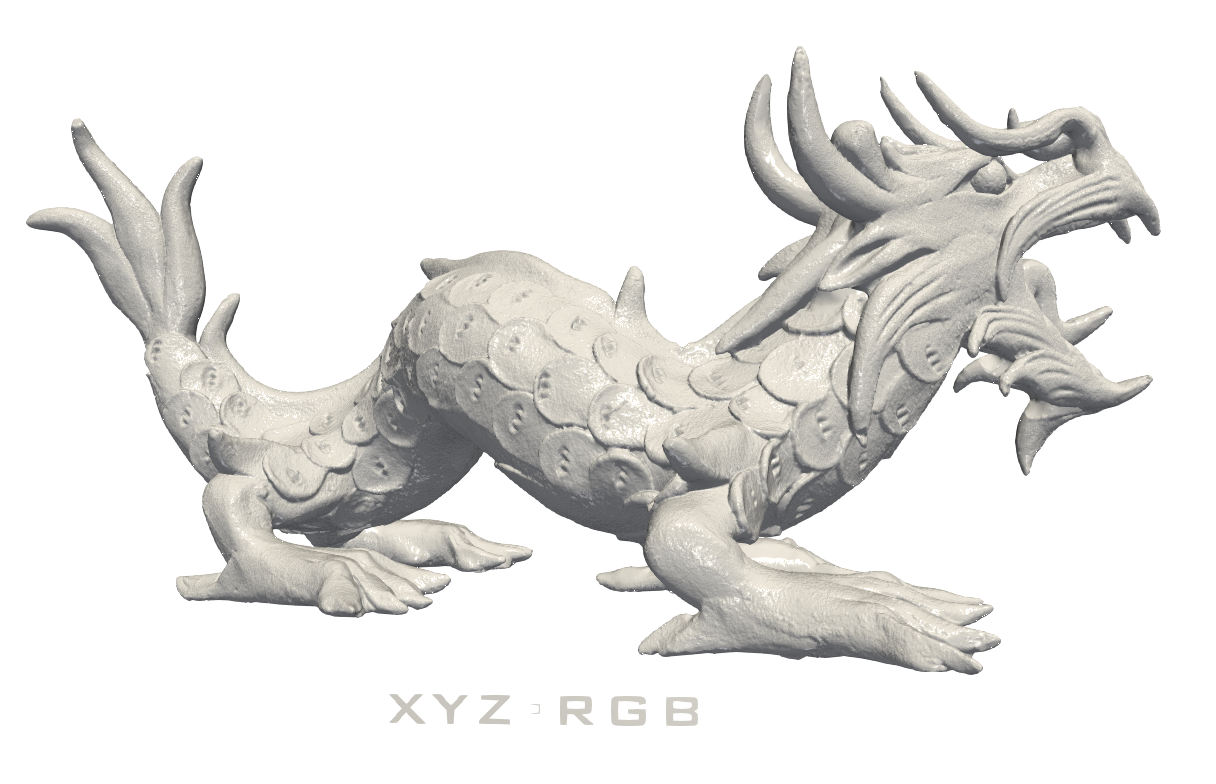
\includegraphics[width=\linewidth]{Asian_Dragon/asian_dragon}
  \caption{Entire dataset, visualised with \textit{surface}  \\
  representation, solid \texttt{\#ffffff} colour and 100\% \\ specular lightning}
\end{subfigure}%
\begin{subfigure}{.5\textwidth}
  \centering
  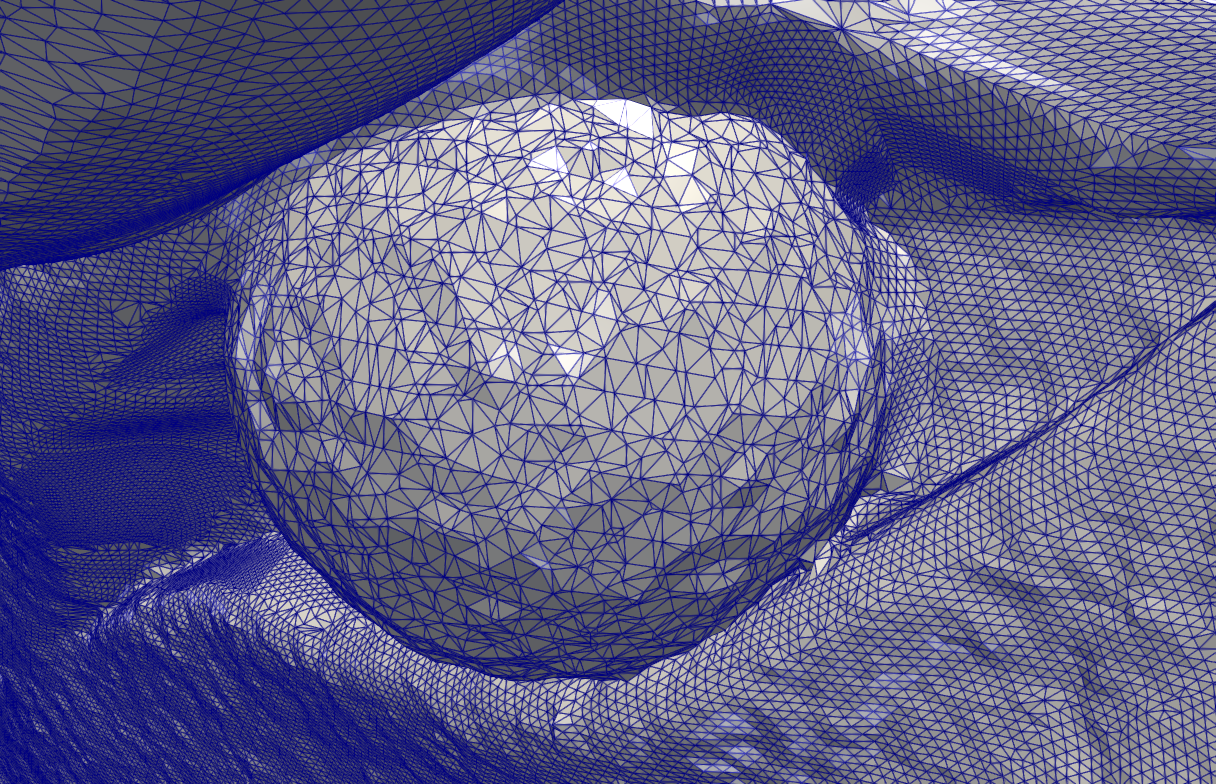
\includegraphics[width=\linewidth]{Asian_Dragon/eye_detail_edges}
  \caption{Eye detail to show the mesh, with \textit{surface with edges} representation, \texttt{\#000080} colour edges}
\end{subfigure}
%\caption{Errore relativo in funzione della dimensione del problema}
\end{figure}










































\end{document}